%% LaTeX-Beamer template for KIT design
%% by Erik Burger, Christian Hammer
%% title picture by Klaus Krogmann
%%
%% version 2.1
%%
%% mostly compatible to KIT corporate design v2.0
%% http://intranet.kit.edu/gestaltungsrichtlinien.php
%%
%% Problems, bugs and comments to
%% burger@kit.edu

\documentclass[18pt]{beamer}

%% SLIDE FORMAT

% use 'beamerthemekit' for standard 4:3 ratio
% for widescreen slides (16:9), use 'beamerthemekitwide'

\usepackage{templates/beamerthemekit}
% \usepackage{templates/beamerthemekitwide}

\usepackage[utf8]{inputenc}
\usepackage{hyperref}
\usepackage{listings}
\usepackage{xcolor}
\usepackage{colortbl}

\definecolor{lime}{HTML}{8FFF53}

%% TITLE PICTURE

% if a custom picture is to be used on the title page, copy it into the 'logos'
% directory, in the line below, replace 'mypicture' with the
% filename (without extension) and uncomment the following line
% (picture proportions: 63 : 20 for standard, 169 : 40 for wide
% *.eps format if you use latex+dvips+ps2pdf,
% *.jpg/*.png/*.pdf if you use pdflatex)

\titleimage{greendrop}

%% TITLE LOGO

% for a custom logo on the front page, copy your file into the 'logos'
% directory, insert the filename in the line below and uncomment it

%\titlelogo{mylogo}

% (*.eps format if you use latex+dvips+ps2pdf,
% *.jpg/*.png/*.pdf if you use pdflatex)

%% TikZ INTEGRATION

% use these packages for PCM symbols and UML classes
% \usepackage{templates/tikzkit}
% \usepackage{templates/tikzuml}

% the presentation starts here

\title[Arrays, Sichtbarkeit, Typ-Konvertierung]{Programmieren:\\ Arrays, Sichtbarkeit, Typ-Konvertierung}
\subtitle{Tutorium 30}
\author{YouniS Bensalah}
\date{November 20, 2015}

\institute{Chair for Software Design and Quality}

% Bibliography

\usepackage[citestyle=authoryear,bibstyle=numeric,hyperref,backend=biber]{biblatex}
\addbibresource{templates/example.bib}
\bibhang1em

\begin{document}

% change the following line to "ngerman" for German style date and logos
\selectlanguage{english}

%title page
\begin{frame}
\titlepage
\end{frame}

%table of contents
\begin{frame}{Heute}
\tableofcontents
\end{frame}

\begin{frame}{Java 8}
    \center
    \Huge{Der Praktomat kann jetzt\\ Java 8 !}
\end{frame}

\section{Arrays}

\subsection{Definition}

\begin{frame}{Array}
    \begin{block}{Array}
        \begin{itemize}
            \item Ein \textbf{Array} ist eine Datenstruktur,
            die eine endliche Folge von Elementen desselben Typs darstellt
            \item Der Zugriff auf ein einzelnes Element erfolgt über einen ganzzahligen \textbf{Index}
        \end{itemize}
    \end{block}
\end{frame}

\begin{frame}{Array}

    \center
    \begin{tabular}{ cccccccc }
        \hline
        \rowcolor{lime}
        \multicolumn{1}{|c|}{7} &
        \multicolumn{1}{c|}{16} &
        \multicolumn{1}{c|}{3} &
        \multicolumn{1}{c|}{-1} &
        \multicolumn{1}{c|}{9} &
        \multicolumn{1}{c|}{32} &
        \multicolumn{1}{c|}{4} &
        \multicolumn{1}{c|}{2}\\
        \hline
        0 & 1 & 2 & 3 & 4 & 5 & 6 & 7\\
    \end{tabular}

    \pause

    \begin{itemize}
        \item Länge: 8
        \item Index: von 0 bis 7
    \end{itemize}

\end{frame}

\begin{frame}[fragile]{Array-Deklaration}
    \begin{exampleblock}{Deklaration und Initialisierung}
        \begin{lstlisting}[language=Java]
int[] myArray = new int[8];
        \end{lstlisting}
    \end{exampleblock}

\end{frame}

\begin{frame}[fragile]{Zugriff auf Array}
    \begin{exampleblock}{Zugriff auf Elemente des Arrays}
        \begin{lstlisting}[language=Java]
myArray[0] = 7;
myArray[1] = 16;
myArray[2] = 3;
myArray[3] = -1;
myArray[4] = 9;
myArray[5] = 32;
myArray[6] = 4;
myArray[7] = 2;
        \end{lstlisting}
    \end{exampleblock}

\end{frame}

\begin{frame}[fragile]{Achtung !}
    \begin{alertblock}{Ein beliebter Fehler}
        \begin{lstlisting}[language=Java]
int[] myArray = new int[8];
myArray[8] = 42;  // nope
        \end{lstlisting}

    \end{alertblock}

    \pause

    \begin{itemize}
        \item Die Indizes gehen von \texttt{0} bis \texttt{7}
        \item Index \texttt{8} wäre das 9. Element !
    \end{itemize}

\end{frame}

\begin{frame}[fragile]{Curly Braces Syntax: \{\}}
    Java erlaubt es, gleich die Elemente des Arrays zu initialisieren.
    \begin{exampleblock}{Curly Braces Syntax}
        \begin{lstlisting}[language=Java]
int[] myArray = {7, 16, 3, -1, 9, 32, 4, 2};
        \end{lstlisting}

    \end{exampleblock}

\end{frame}

\begin{frame}[fragile]{Was kommt raus \dots}
    \begin{lstlisting}[language=Java,basicstyle=\scriptsize]
int[] x = new int[4];

x[0] = 1;
x[1] = x[0] + x[0];
x[2] = x[1] + x[1] + x[1] + x[1];
x[3] = x[2] + x[2] + x[2] + x[2] + x[2] + x[2] + x[2] + x[2];

System.out.println(x[3]);
    \end{lstlisting}

\end{frame}

\begin{frame}{Was kommt raus \dots}
    \begin{exampleblock}{Ausgabe}
        64
    \end{exampleblock}
\end{frame}


\begin{frame}[fragile]{Was kommt raus \dots}
    \begin{lstlisting}[language=Java,basicstyle=\scriptsize]
int[] m = new int[5];

m[0]                = 1;
m[m[0]]             = m[0] + m[0];
m[m[m[0]]]          = m[0] + m[m[0]];
m[m[m[m[0]]]]       = m[m[0]] + m[m[m[0]]] - m[0];
m[m[m[m[m[0]]]]]    = m[0] + m[m[0]] + m[m[m[0]]] + m[m[m[m[0]]]];

System.out.println(m[m[m[m[m[0]]]]]);
    \end{lstlisting}

\end{frame}

\begin{frame}{Was kommt raus \dots}
    \begin{exampleblock}{Ausgabe}
        10
    \end{exampleblock}
\end{frame}

\begin{frame}[fragile]{Was kommt raus \dots}
    \begin{lstlisting}[language=Java,basicstyle=\scriptsize]
int[] h = new int[3];

h[0] = 1;
h[1] = 2;
h[2] = h[0] + h[1];
h[3] = h[0] + h[1] + h[2];

System.out.println(h[3]);
    \end{lstlisting}

\end{frame}

\begin{frame}[fragile]{U MAD?}
    \begin{alertblock}{Ausgabe}
        \alert{Exception in thread "main" java.lang.ArrayIndexOutOfBoundsException}
    \end{alertblock}

\pause

    \textbf{Index \texttt{3} gehört nicht zum Array \texttt{h[]} !}

\begin{exampleblock}{}
    \begin{lstlisting}[language=Java]
int[] h = new int[3];
// ...
// index 3 is out of bounds!
h[3] = h[0] + h[1] + h[2];
    \end{lstlisting}
\end{exampleblock}

\end{frame}

\subsection{Länge eines Arrays}

\begin{frame}[fragile]{Länge eines Arrays}
    Man kann die Länge eines beliebigen Arrays mit dem Attribut \texttt{length} ermitteln.


\begin{exampleblock}{}
    \begin{lstlisting}[language=Java]
String[] names = {"Tick", "Trick", "Track"};

int count = names.length;  // 3
    \end{lstlisting}
\end{exampleblock}

\end{frame}

\subsection{Iteration über Array}

\begin{frame}[fragile]{Iteration über Array: for}
    \begin{itemize}
        \item Wir möchten nun über einen Array \textbf{interieren} \dots
        \item Idee: \texttt{for}-Schleife mit Zählvariable als Index
    \end{itemize}

    \begin{exampleblock}{for-Schleife über Array}
        \begin{lstlisting}[language=Java]
int[] a = new int[128];

for (int i = 0; i < a.length; i++) {
    a[i] = (int)(Math.random() * i);
}
        \end{lstlisting}

    \end{exampleblock}

\end{frame}

\begin{frame}{Iteration über Array: for}
    \textbf{for-Schleife}
    \begin{itemize}
        \item Vorteile
        \begin{itemize}
            \item Flexible Grenzen
            \item Index innerhalb der Schleife verwendbar
            \item Schleife über mehrere Arrays gleichzeitig möglich

        \end{itemize}
        \pause
        \item Nachteile
        \begin{itemize}
            \item Man muss jedes Mal Anfang und Ende des Index explizit angeben
            \item Index interessiert oft nicht
            \item Fehleranfällig: Index könnte durch Fehler aus dem Array rauslaufen (daher auf jeden Fall \texttt{length} verwenden)
        \end{itemize}
    \end{itemize}
\end{frame}

\begin{frame}[fragile]{Iteration über Array: foreach}
    Java kennt eine spezielle Variante von \texttt{for}:\\


    \begin{exampleblock}{foreach-Schleife über Array}
        \begin{lstlisting}[language=Java]
String[] b = new String[256];

for (String e : b) {
    System.out.println(e);
}
        \end{lstlisting}

    \end{exampleblock}
\end{frame}

\begin{frame}{Iteration über Array: foreach}
    \textbf{foreach-Schleife}
    \begin{itemize}
        \item Vorteile
        \begin{itemize}
            \item Einfache Syntax
            \item Kein Index, kann also niemals durch Fehler aus Array rauslaufen
            \item Schleife über mehrere Arrays gleichzeitig möglich

        \end{itemize}
        \pause
        \item Nachteile
        \begin{itemize}
            \item Man kann bei Array von primitiven Datentypen (int, double,\dots) die Werte nicht verändern
            \item Index nicht mehr in Schleifenrumpf bekannt
            \item Iteriert immer über ganzen Array
        \end{itemize}
    \end{itemize}
\end{frame}

\begin{frame}[fragile]{Was kommt raus \dots}
    \begin{lstlisting}[language=Java]
int[] v = new int[11];

v[0] = 2;

for (int i = 1; i < v.length; i++) {
    v[i] += v[i-1] + 4;
}

System.out.println(v[10]);
    \end{lstlisting}

\end{frame}

\begin{frame}{Was kommt raus \dots}
    \begin{exampleblock}{Ausgabe}
        42
    \end{exampleblock}
\end{frame}

\begin{frame}[fragile]{Was kommt raus \dots}
    \begin{lstlisting}[language=Java,basicstyle=\scriptsize]
int s = 0;

int[] s1 = new int[100];
int[] s2 = new int[100];

for (int i = 0; i < s1.length; i++) {
    s1[i] = i+1;
    s2[s2.length - 1 - i] = s1[i];
}

for (int i = 0; i < s1.length; i++) {
    s += s1[i] + s2[i];
}

s /= 2;

System.out.println(s);
    \end{lstlisting}

\end{frame}

\begin{frame}{Was kommt raus \dots}
    \begin{exampleblock}{Ausgabe}
        5050
    \end{exampleblock}
\end{frame}

\begin{frame}[fragile]{Was kommt raus \dots}
    \begin{lstlisting}[language=Java,basicstyle=\scriptsize]
int n = 10;
String[] w = new String[5*n];

for (int i = 0; i < w.length; i++) {
    if (i % 5 == 0) {
        for (int j = 0; j < 5 && i+j < w.length; j++) {
            if (j % 2 == 0) {
                w[i+j] = "V";
            } else {
                w[i+j] = "A";
            }
        }
        w[i] = "J";
    } else if (i % 5 % 4 == 0) {
        w[i] = " ! \n";
    }
}

for (String e : w) {
    System.out.print(e);
}
    \end{lstlisting}

\end{frame}

\begin{frame}{Was kommt raus \dots}
    \begin{exampleblock}{Ausgabe}
        JAVA !\\
        JAVA !\\
        JAVA !\\
        JAVA !\\
        JAVA !\\
        JAVA !\\
        JAVA !\\
        JAVA !\\
        JAVA !\\
        JAVA !
    \end{exampleblock}
\end{frame}

\subsection{Mehrdimensionale Arrays}

\begin{frame}{Mehrdimensionale Arrays}
    \begin{itemize}
        \item Ein mehrdimensionales Array ist als \textit{"Array von Arrays"} zu verstehen
        \item n-dimensionales Array hat n Indizes
        \item Ein 2D Array kann z.B. als Matrix aufgefasst werden
    \end{itemize}
\end{frame}

\begin{frame}[fragile]{Mehrdimensionale Arrays}
    \begin{exampleblock}{Code-Beispiel}
        \begin{lstlisting}[language=Java]
int[][] matrix = new int[4][6];  // 4x6 matrix

matrix[0][1] = 7;
matrix[1][0] = 8;
matrix[3][5] = 9;
        \end{lstlisting}

    \end{exampleblock}

\end{frame}

\begin{frame}[fragile]{Mehrdimensionale Arrays}
    \begin{itemize}
        \item Wie iteriert man über ein mehrdimensionales Array ?
        \pause
        \item \textbf{Geschachtelte \texttt{for}-Schleifen !}
    \end{itemize}


    \begin{exampleblock}{Code-Beispiel}
        \begin{lstlisting}[language=Java]
int[][] matrix = new int[4][6];

for (int i = 0; i < matrix.length; i++) {
    for (int j = 0; j < matrix[i].length; j++) {
        matrix[i][j] = i + j;
    }
}
        \end{lstlisting}

    \end{exampleblock}

\end{frame}

\begin{frame}[fragile]{Was kommt raus \dots}
    \begin{lstlisting}[language=Java,basicstyle=\scriptsize]
int[][] m = new int[3][3];

for (int i = 0; i < m.length; i++) {
    for (int j = 0; j < m[i].length; j++) {
        if (i == j) {
            m[i][j] = 1;
        } else {
            m[i][j] = 0;
        }
    }
}

for (int[] x : m) {
    for (int y : x) {
        System.out.print(y + " ");
    }
    System.out.print("\n");
}
    \end{lstlisting}

\end{frame}

\begin{frame}{Was kommt raus \dots}
    \begin{exampleblock}{Ausgabe}
        1 0 0\\
        0 1 0\\
        0 0 1
    \end{exampleblock}
\end{frame}

\begin{frame}{Arrays wie Objekte in Java}
    \begin{alertblock}{Arrays wie Objekte in Java}
        \begin{itemize}
            \item Arrays werden in Java wie Objekte behandelt !
            \item \texttt{int[] a = \{1, 2, 3\};} erstellt ein neues Array und weist \texttt{a} die Referenz auf das Array zu
            \item Nach \texttt{int[] b = a;} referenzieren \texttt{a} und \texttt{b} \textbf{dasselbe} Array !
            \item Nach \texttt{b[1] = 42;} wertet \texttt{a[1]} zu \texttt{42} aus
        \end{itemize}

    \end{alertblock}

\end{frame}

\section{Typ-Konvertierung}

\begin{frame}{Typ-Konvertierung}
    \begin{block}{Widening Primitive Conversions}
        \begin{itemize}
            \item \textbf{Kein Informationsverlust} bzgl. der \textbf{Größe}
            \item \alert{\textbf{Informationsverlust}} hinsichtlich \alert{\textbf{Präzision}} möglich
            \item Automatisch (kein expliziter Cast erforderlich)
        \end{itemize}
    \end{block}

\end{frame}

\begin{frame}[fragile]{Typ-Konvertierung}
    \begin{block}{Narrowing Primitive Conversions}
        \begin{itemize}
            \item \alert{\textbf{Informationsverlust}} bzgl. der \alert{\textbf{Größe}} möglich
            \item \alert{\textbf{Informationsverlust}} hinsichtlich \alert{\textbf{Präzision}} möglich
            \item Bei ganzzahligen Typen werden höherwertige Bits abgeschnitten
            \item Cast-Operator notwendig:
            \begin{lstlisting}[language=Java,basicstyle=\scriptsize]
int x = 2000;
byte b = (byte)x;  // -48
            \end{lstlisting}

        \end{itemize}
    \end{block}

\end{frame}

\begin{frame}[fragile]{Typ-Konvertierung}
    \begin{block}{String Conversions}
        \begin{itemize}
            \item Jeder Datentyp kann nach String konvertiert werden
            \item Für primitive Typen geschieht dies automatisch
            \item Für Klassen kann man eine eigene \texttt{toString} Methode angeben
            \begin{lstlisting}[language=Java,basicstyle=\scriptsize]
class Vector2D {
    double x, y;

    public String toString() {
        return "(" + x + ", " + y + ")";
    }
}
            \end{lstlisting}

        \end{itemize}
    \end{block}

\end{frame}

\begin{frame}[fragile]{Was macht diese Methode \dots}
    \begin{lstlisting}[language=Java]
public int x(int a, int b) {
    return (int)((b - a + 1) * Math.random()) + a;
}
    \end{lstlisting}


    \vspace{.5in}
    Was gibt \texttt{x(a, b)} zurück ?

\end{frame}

\begin{frame}{Was macht diese Methode \dots}
    \begin{exampleblock}{}
        \texttt{x(a, b)} berechnet ganzzahligen Zufallswert zwischen \texttt{a} und \texttt{b} (inklusive).
    \end{exampleblock}
\end{frame}

\section{Sichtbarkeit}

\subsection{Datenkapselung}

\begin{frame}{Datenkapselung}
    \begin{itemize}
        \item Ermöglicht Verbergen von Daten
        \item Details der Implementierung nicht nach außen sichtbar
        \item Weniger Abhängigkeiten zwischen Klassen
        \item Genau festgelegte Schnittstelle
    \end{itemize}
\end{frame}

\subsection{Sichtbarkeitsmodifizierer}

\begin{frame}{Public vs Private}

    Sichtbarkeitsmodifizierer in Java (\texttt{public}, \texttt{private} \dots) können auf \textbf{Attribute}, \textbf{Methoden} und \textbf{Klassen} angewandt werden.
    \begin{itemize}
        \item \texttt{public}
        \begin{itemize}
            \item Nach außen sichtbar
        \end{itemize}
        \item \texttt{private}
        \begin{itemize}
            \item Nur von innen sichtbar
        \end{itemize}
    \end{itemize}
\end{frame}

\begin{frame}{Richtlinie}
    \begin{itemize}
        \item Attribute sollten immer \textbf{private} sein !
        \item \textbf{Getter} \& \textbf{Setter} verwenden
        \item Hilfsmethoden auch \textbf{private}
        \item Nur Schnittstelle ist \textbf{public}
    \end{itemize}
\end{frame}


\appendix
\beginbackup

\begin{frame}{Fragen ?}
    \begin{figure}
        
\includegraphics[scale=.3]{img/fragen.jpg}
    \end{figure}
\end{frame}

\begin{frame}{Bis nächste Woche !}
    \begin{figure}
        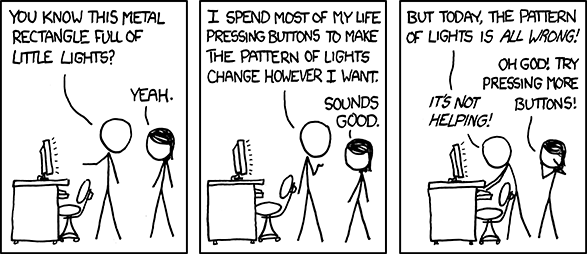
\includegraphics[scale=.5]{img/computer_problems.png}
    \end{figure}

    \begin{flushright}
    \footnotesize{xkcd.com}
    \end{flushright}
\end{frame}

\backupend

\end{document}
